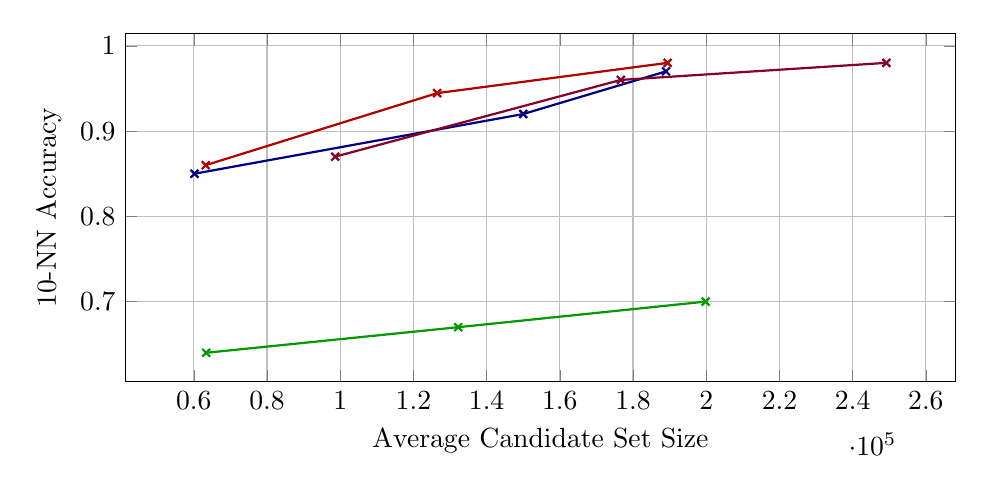
\begin{tikzpicture}
        \begin{axis}[
            width=\linewidth,
            height=6cm,
            grid=major,
            xlabel={Average Candidate Set Size},
            ylabel={10-NN Accuracy},
            mark options={solid}
        ]
        
        % Original
        \addplot[blue!50!black, thick, mark=x, mark size=2pt] coordinates {
            (60200, 0.85)
            (150000, 0.92)
            (189000, 0.97)
        };
        % PCA
        \addplot[red!70!black, thick, mark=x, mark size=2pt] coordinates {
            (63243, 0.86)
            (126475, 0.9445)
            (189444, 0.98)
        };
        % Mahalanobis
        \addplot[green!60!black, thick, mark=x, mark size=2pt] coordinates {
            (63386, 0.64)
            (132219, 0.67)
            (199818, 0.70)
        };
        % Multi-model ensembling 
        \addplot[purple!70!black, thick, mark=x, mark size=2pt] coordinates {
            (98631, 0.87)
            (176668, 0.96)
            (249204, 0.98)
        };
        \end{axis}
\end{tikzpicture}